\chapter{Conclusion and Future work}\label{C:con}

\section{Conclusion}

In the project we first developed a model for serivce location-allocation problem so that it can be 
tackled by evolutionary multi-objective optimization (EMO). Secondly, we developed a multi-objective PSO-based 
algorithm to solve the problem. The experiments show that our algorithm is both effecient and effective than 
NSGA-II based algorithm. One of challenge is to find a proper for the value of the 
transformation threshold. There is no systematic approach to determine the optimal transformation
threshold. In order to solve this problem, we mainly consider a binary-based PSO (BPSO) approach. It is natural to apply BPSO
on a binary-based representation, therefore BPSO and NSGA-II could use the same representation. 
In the future, we will  further investigate the impact of the parameter settings of
multi-objective PSO and developed a single-objective binary PSO to compare with multi-objective based PSO.

A Gantt chart showing the brief plan for the rest of the project is illustrated as follows.
\begin{figure}[h!]
	\centering
	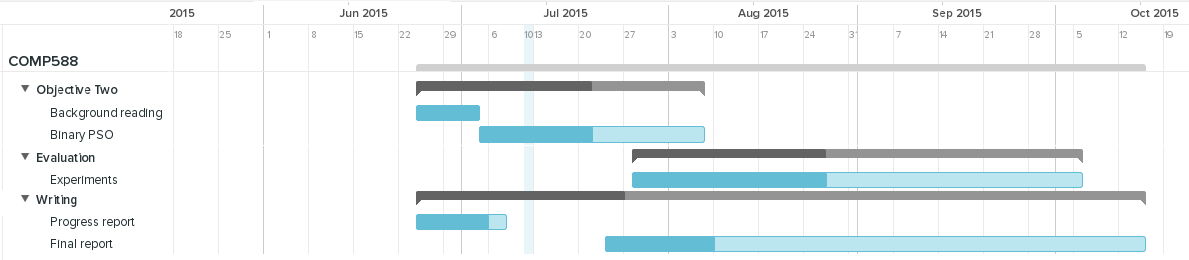
\includegraphics[width=1\textwidth]{pics/timetable.png}
	\caption{A Gantt chart for the rest of the project}
\end{figure}


